% Gemini theme
% https://github.com/anishathalye/gemini

\documentclass[final, 16pt]{beamer}

% ====================
% Packages
% ====================
%\usepackage[x11names]{xcolor} % use color for the horizontal line
\usepackage[T1]{fontenc}
\usepackage{lmodern}
\usepackage[size=custom,width=38.1,height=54.2,scale=0.4]{beamerposter}
\usetheme{gemini}
\usecolortheme{gemini}
\usepackage{graphicx}
\usepackage{booktabs}
\usepackage{tikz}
\usepackage{pgfplots}
\usepackage[square,sort,comma,numbers]{natbib} % for simplify the format of the references
\usepackage{tikz} % for adding the logo
% \usepackage{caption} % for caption font of the table
\setbeamertemplate{caption}[numbered]
\setbeamerfont{caption}{size=\large}

% ====================
% Lengths
% ====================

% If you have N columns, choose \sepwidth and \colwidth such that
% (N+1)*\sepwidth + N*\colwidth = \paperwidth
\newlength{\sepwidth}
\newlength{\colwidth}
\setlength{\sepwidth}{0.025\paperwidth}
\setlength{\colwidth}{0.45\paperwidth}

\newcommand{\separatorcolumn}{\begin{column}{\sepwidth}\end{column}}

% ====================
% Title
% ====================

\title{Mining relationships between food groups, eating time slots\\ and diabetes status in adults from UK NDNS RP}

\author{Luigi Palla \inst{1} \and Chaochen Wang \inst{2} \and Suzana Almoosawi \inst{3}}

\institute[shortinst]{\inst{1} Dept Medical Statistics, LSHTM, London, UK; \samelineand \inst{2} Dept Public Health, Aichi Medical University, Aichi, Japan \samelineand \\ \inst{3} Brain, Performance and Nutrition Research Centre, Northumbria University, Newcastle, UK}

% ====================
% Body
% ====================
\pgfplotsset{compat=1.16}
\begin{document}

% logos are added as follows:

\addtobeamertemplate{headline}{} 
{
	\begin{tikzpicture}[remember picture,overlay] 
%	\node [anchor=north east, inner sep=3cm] at (current page.north east) {\includegraphics[height=5cm]{Fig/LSHTM-logo-trans-white.eps}}; 
    \node [anchor=north east, inner sep=3.4cm] at ([xshift=2.5cm,yshift=1.3cm]current page.north east)     {\includegraphics[height=2.5cm]{Fig/LSHTM-logo-trans-white.eps}}; 
	\end{tikzpicture} 
}

\addtobeamertemplate{headline}{} 
{
	\begin{tikzpicture}[remember picture,overlay] 
	%	\node [anchor=north east, inner sep=3cm] at (current page.north east) {\includegraphics[height=5cm]{Fig/LSHTM-logo-trans-white.eps}}; 
	\node [anchor=north west, inner sep=3.7cm] at ([xshift=-2.7cm,yshift=1.5cm]current page.north west) {\includegraphics[height=2.5cm]{Fig/amu-logo-trans-white.eps}}; %{\includegraphics[height=6.6cm]{Fig/amu-logo-trans-green.eps}};  
	\end{tikzpicture} 
}

\addtobeamertemplate{headline}{} 
{
	\begin{tikzpicture}[remember picture,overlay] 
	%	\node [anchor=north east, inner sep=3cm] at (current page.north east) {\includegraphics[height=5cm]{Fig/LSHTM-logo-trans-white.eps}}; 
	\node [anchor=north west, inner sep=3.7cm] at ([xshift=0.5cm,yshift=1.5cm]current page.north west) {
\includegraphics[height=2.5cm]{Fig/suzana-logo-trans-white.eps}}; \end{tikzpicture} 
}



\begin{frame}[t]
\begin{columns}[t]
\separatorcolumn

\begin{column}{\colwidth}
    \vskip-1.45ex
  \begin{block}{Introduction}

    \vskip-1.45ex
    \begin{itemize}
	\item The timing of energy/nutrient intake has been previously shown to be associated with obesity and diabetes \cite{Almoosawi2019Chrono};
	\item Recently derived diurnal patterns of energy/carbohydrate intake suggested the potential interplay of circadian biology and social behaviour contributing to obesity \cite{Palla2019};
	% \item Evening intake of energy is positively associated with incidence of hypertension, and overweight/obesity \cite{Almoosawi2013,almoosawi2016chrono}.
  \item The relationship between food groups and the time when they are eaten is of interest, how such relationships vary by type 2 diabetes status are still left unknown.
\end{itemize}
    % \vskip-1.45ex



% Recent evidence suggested that there are three types of eaters \textbf{(grazers, early eaters, and late eaters)} according to the timing of energy consumption \cite{leech2017temporal,mansukhani2018investigating}. However, the temporal eating patterns were based on averaging the total energy intake  measured in the questionnaires and therefore \textbf{could not capture the day-to-day variation in eating patterns}. Furthermore, most previous studies have focused on describing temporal patterns of energy intake, \textbf{without considering the timing of macro-nutrient intake}.

%    \vskip-1.45ex
%%\begin{itemize}
%	\item 
%	\item 
%	
%%	Besides they were focussed on total energy \textbf{so would not provide any clue of the temporal eating patterns specifically for nutrient intake}.
%	%	\item Shift workers have a higher risk of developing T2D \cite{pan2011rotating}. 
%%\end{itemize}
%\vskip-1.45ex

%%
%However, the temporal eating patterns were based only on averaging the total energy intake measured by 1 or 2 24-hour dietary recalls \cite{leech2017temporal} or 3 to 4 days' diet diary \cite{mansukhani2018investigating} and therefore \textbf{could not capture the day-to-day variation in eating patterns}, and \textbf{neither could it provide any clue of the temporal patterns specifically for nutrient intake}. 

%This is mainly due to limitations in the FFQ often used in observational studies and the lack of understanding of statistical techniques that can capture the complexity of eating patterns across the day. 

% This study aims at finding both time and quantity eating patterns specifically for carbohydrate (CH) intake in UK adults.


  \end{block}


   \vskip-3.85ex
  \begin{block}{Data and Methodology}
    \vskip-1.85ex

\begin{itemize}
	\item National Diet and Nutrition Survey Rolling Programme (NDNS RP, 2008-2017) included 6802 adults (2810 men and 3992 women) aged 19 or older in the UK, and their 749,026 food recordings collected by a 4-day-diary.
	\item Time of the day was categorized into 7 slots: 6-9 am, 9-12 noon, 12-2 pm, 2-5 pm, 5-8 pm, 8-10 pm and 10 pm-6 am.
	\item The derived contingency table between 60 food groups and the above 7 time slots were analyzed by Correspondence Analysis (CA). Biplots separately for the foods included in the food healthiness score  tertiles, for all adults combined and separately by diabetes status.
	
	\item The odds ratio estimate was derived of consuming unhealthy food groups later in the day compared to earlier in the day, by logistic regression.

\end{itemize}
 \vskip-1.85ex
% Please add the following required packages to your document preamble:
% \usepackage{booktabs}
\begin{table}
% \captionsetup{font=large}
\centering
% \captionof{table}{Definition of Type 2 Diabetes.} \label{tab:title2} 
\caption{\label{tab:tab1}Definition of Type 2 Diabetes.}
\vskip-1.85ex
\begin{tabular}{lccc}
\toprule
\textbf{Diabetes status} & \textbf{Self-reported} & \textbf{Glucose (mmol/L)} & \textbf{HbA1c (\%)} \\ \midrule
No diabetes              & No                     & $<$ 6.10             & $<$ 6.5       \\
Pre-diabetes             & No                     & 6.10 $\sim$ 6.99            & --                  \\
Undiagnosed              & No                     & $\geqslant$ 7.00      & $\geqslant$ 6.5 \\
Diagnosed                & Yes                    & --                        & --                  \\ \bottomrule
\end{tabular}
\end{table}
\vskip-1.45ex




  \end{block}

\vskip-2.45ex
  \begin{block}{Results}
\vskip-2.45ex
    \begin{figure}
      \centering
      \caption{Biplot for CA of 60 food groups and 7 time slots in NDNS RP, among non-diabetes.}
      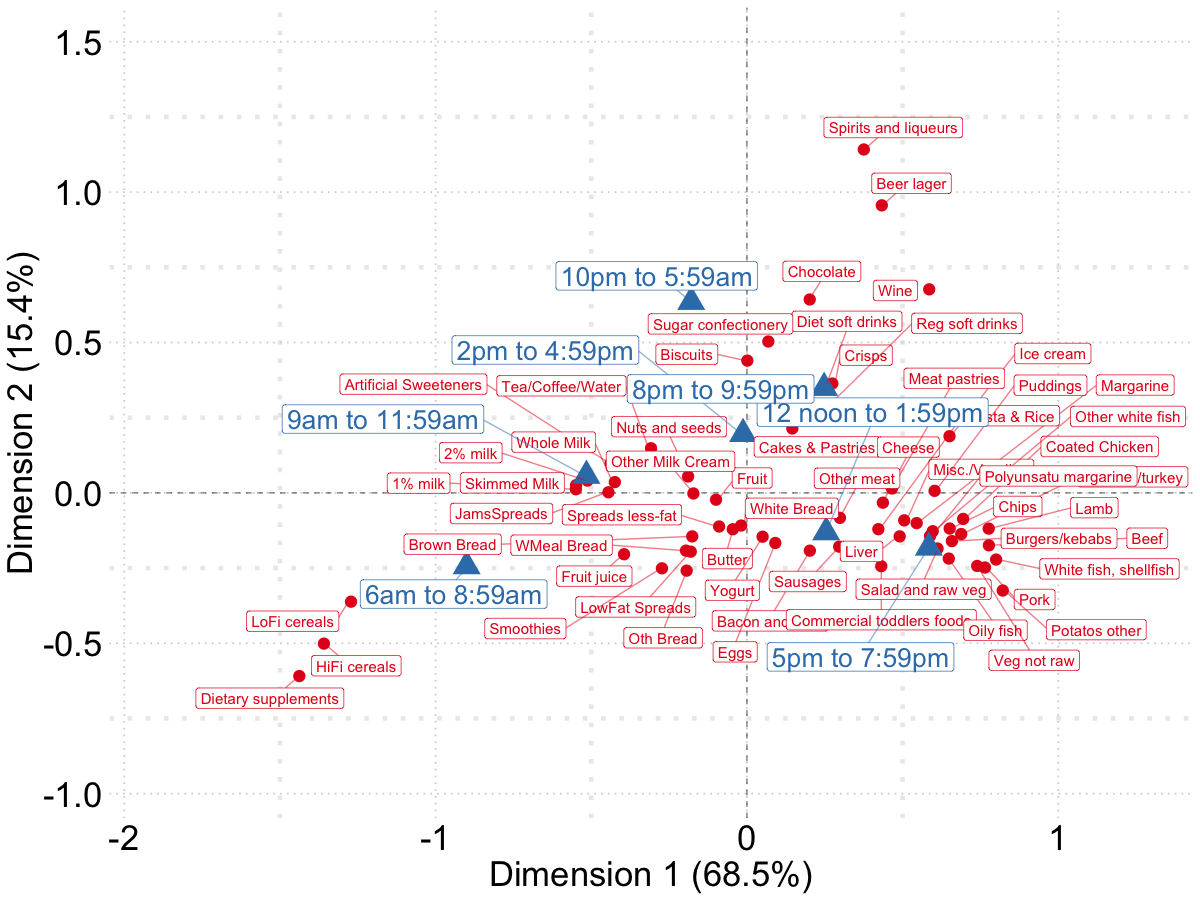
\includegraphics[width=0.88\textwidth]{Fig/F60T7_nonDM.png}	\vskip-2.45ex
      \label{fig:NonDM}
    \end{figure}
\vskip-1ex

\begin{figure}
      \centering
      \caption{Biplot for CA of 60 food groups and 7 time slots in NDNS RP, among diabetes.}
      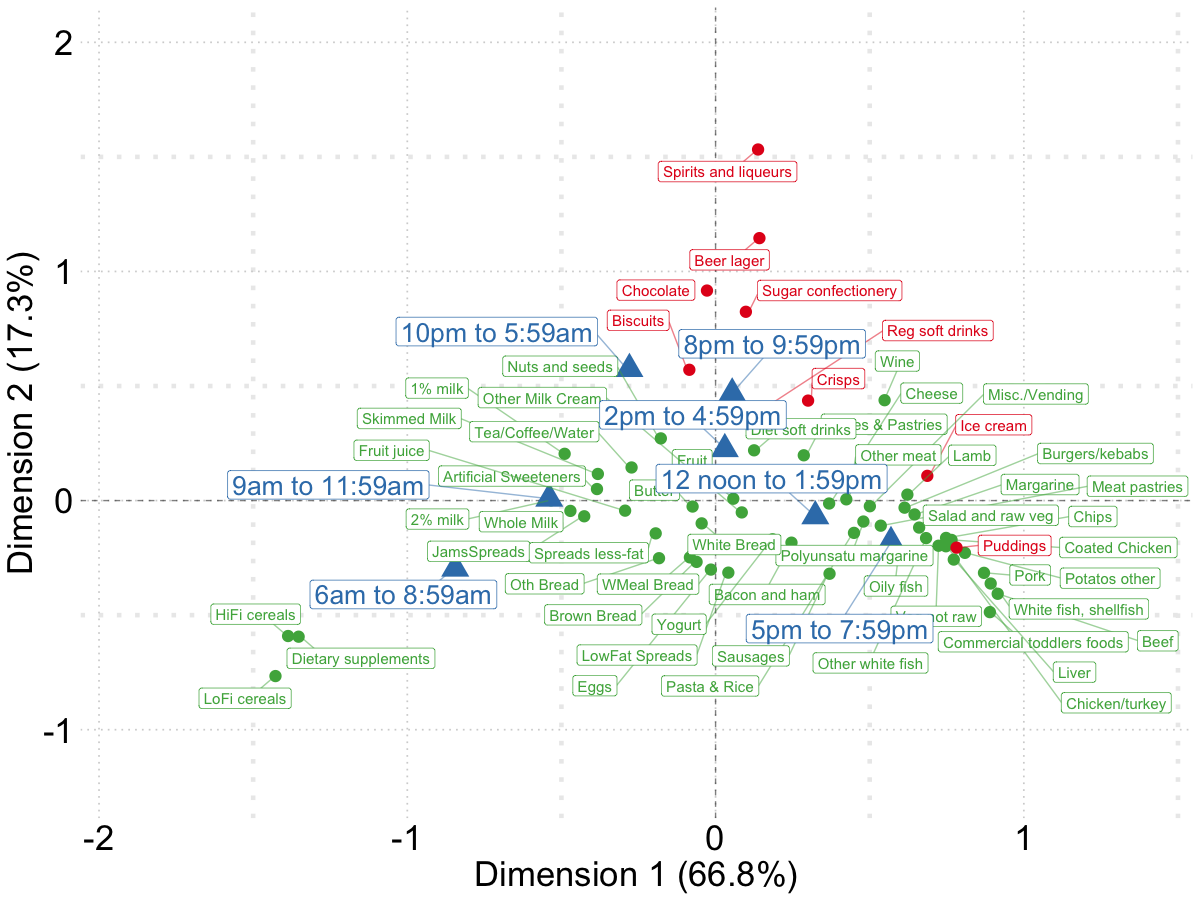
\includegraphics[width=0.88\textwidth]{Fig/F60T7_DM.png}	\vskip-2.45ex
      \label{fig:DM}
    \end{figure}
    
  \end{block}

\end{column}

\separatorcolumn

\begin{column}{\colwidth}
  \begin{block}{}

    \begin{figure}
      \centering
      \caption{Biplot for CA of 60 food groups and 7 time slots in NDNS RP, among undiagnosed diabetes.}
      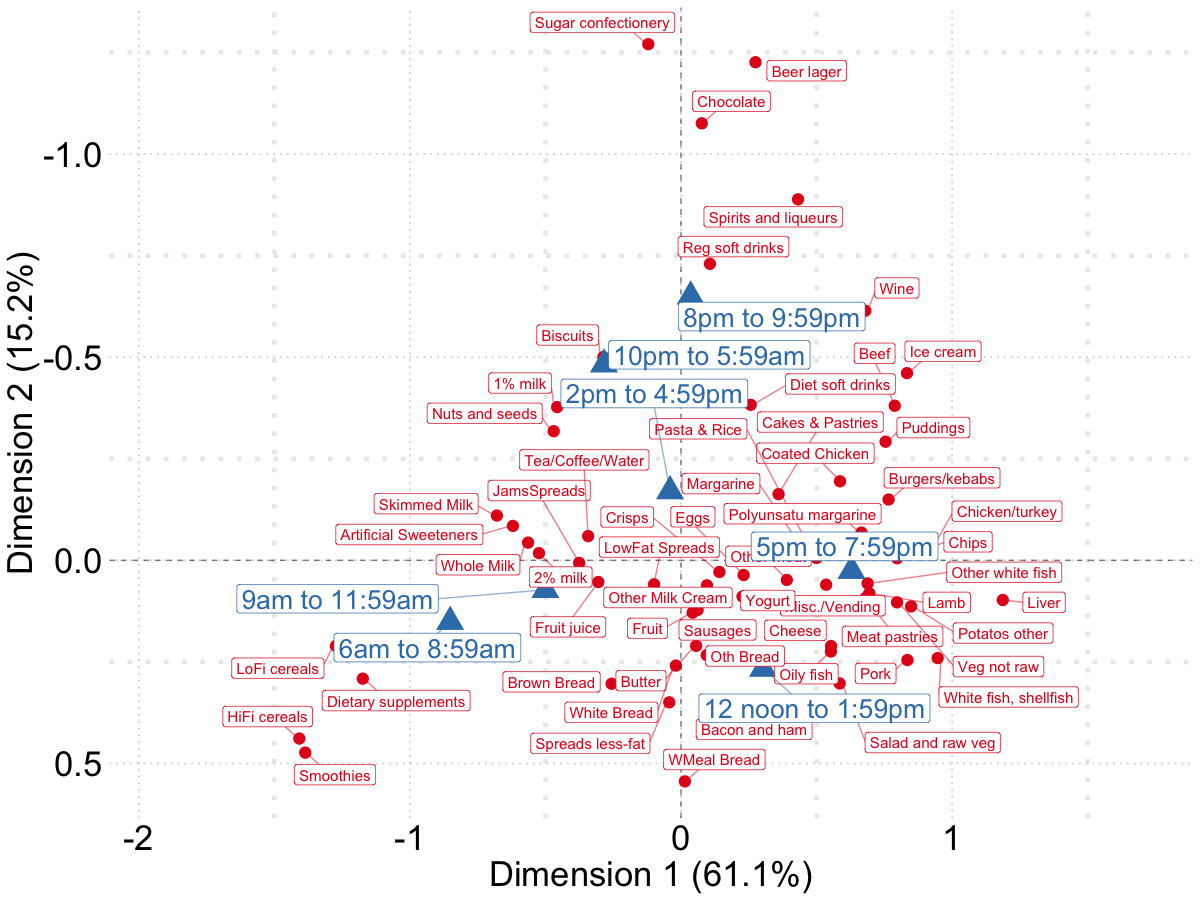
\includegraphics[width=0.88\textwidth]{Fig/F60T7_UndiagDM.png}	\vskip-2.45ex
      \label{fig:UndiagDM}
    \end{figure}
    \begin{figure}
      \centering
      \caption{Biplot for CA of 60 food groups and 7 time slots in NDNS RP, among pre-diabetes.}
      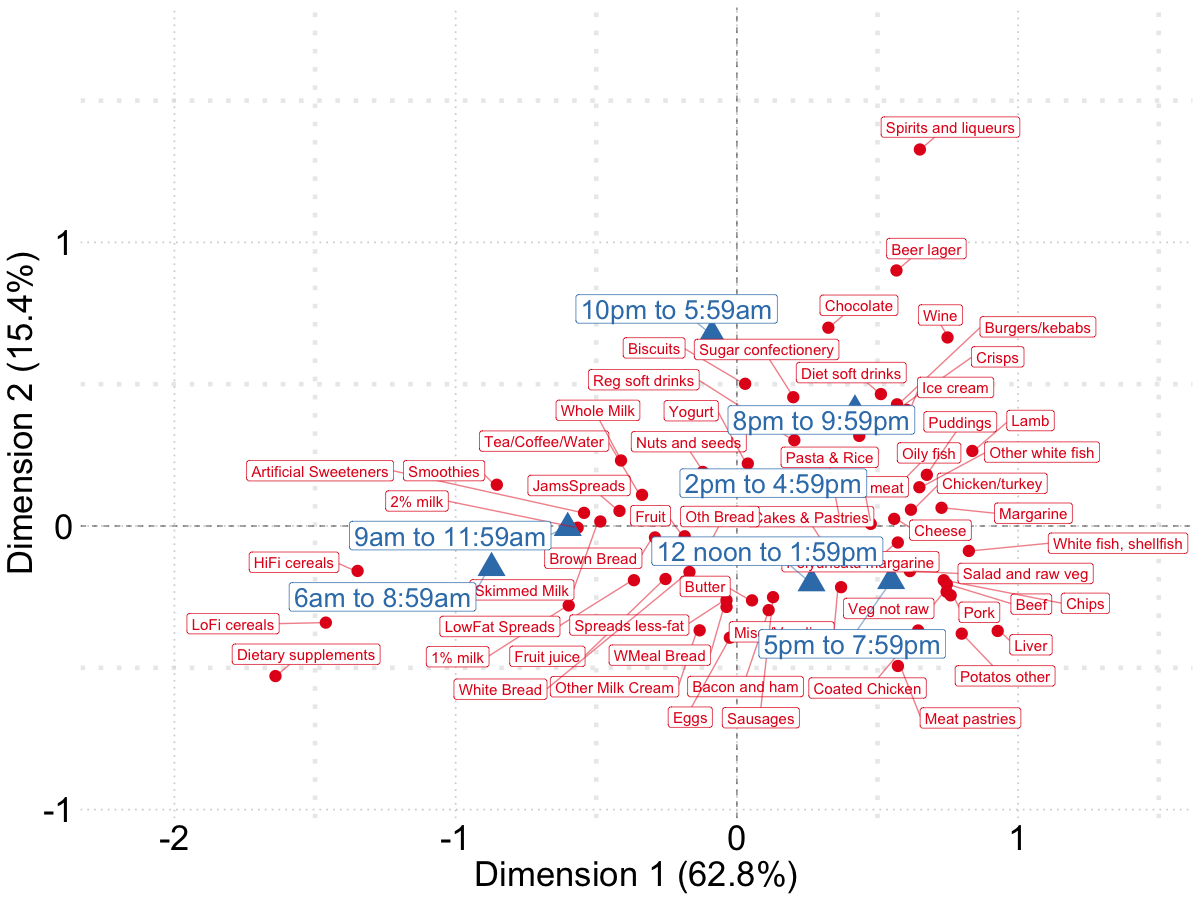
\includegraphics[width=0.88\textwidth]{Fig/F60T7_PreDM}	\vskip-2.45ex
      \label{fig:PreDM}
    \end{figure}
    % \begin{figure}
    %   \centering
    %   \caption{Biplot for CA of 60 food groups and 7 time slots in NDNS RP.}
    %   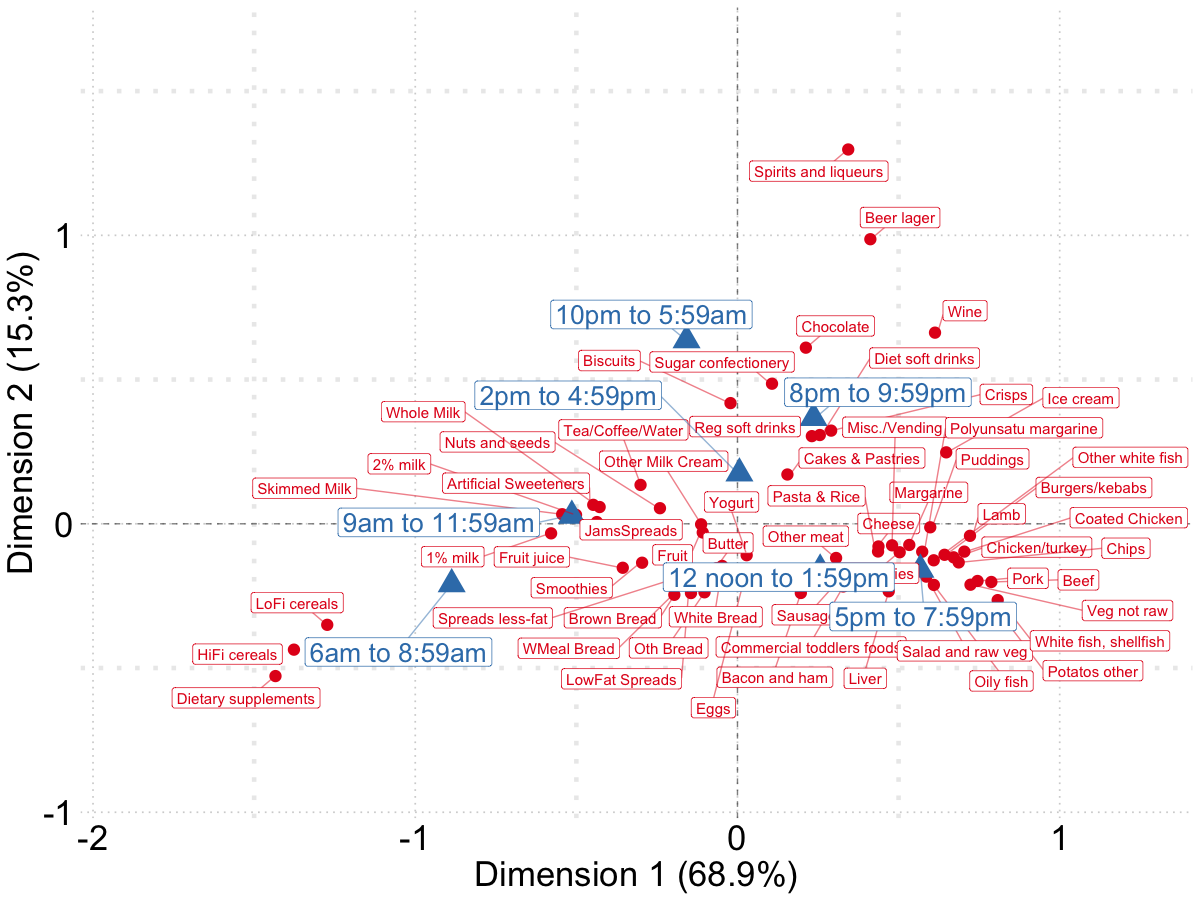
\includegraphics[width=0.95\textwidth]{Fig/F60T7.png}	\vskip-2.45ex
    %   \label{fig:PreDM}
    % \end{figure}
  \end{block}



\begin{block}{Discussion}

\end{block}


\end{column}

\separatorcolumn
\end{columns}



% \someheading{Discussion}
% \par
% \begingroup
% \leftskip2em
% \rightskip\leftskip
% \somebody{The high-CH eaters profile seemed to be the healthiest. Low-CH eating which was crudely associated with higher prevalence of hypertension and obesity may have resulted from health/weight concerns, leading to fat or alcohol as replacements for CH. To ascertain the direction of causality in the association of CH patterns with blood pressure and obesity, prospective longitudinal studies are warranted. }
% \par
% \endgroup

\noindent\textcolor{steelblue}{\rule{\textwidth}{0.4pt}}
%  \begin{block}{References}
    \vskip-1.25ex
%    \nocite{*}
    \footnotesize{\bibliographystyle{elsarticle-num}\bibliography{poster}}

%  \end{block}

%\end{column}
%
%\separatorcolumn
%\end{columns}
%\end{frame}
\end{frame}
\end{document}
